\chapter{Comparison between Nonlinear Model and Real System Pendulum Behavior}\label{comparisonModelReal} 
\textbf{Name: Group 630}\\
\textbf{Date: 11/03 - 2016}

\subsubsection{Purpose}
Compare the response of the real setup when hanging upside down with the simulation given by the theoretical nonlinear model.

\subsubsection{Setup}
\fxnote{Include image of the setup}
\subsubsection{Procedure}
\begin{enumerate}
	\item Turn on the power supply
	\item Place the setup upside-down and place the frame touching the base, \si{135^0} with respect to the vertical position
	\item Use the oscilloscope to measure the changes in the potentiometer 
	\item Let the Cubli fall
	\item Collect all the data and plot it in Matlab
	\item Compare with the simulation 
	
\end{enumerate}

\subsubsection{Results}
\begin{figure}[H] 
	\centering 
	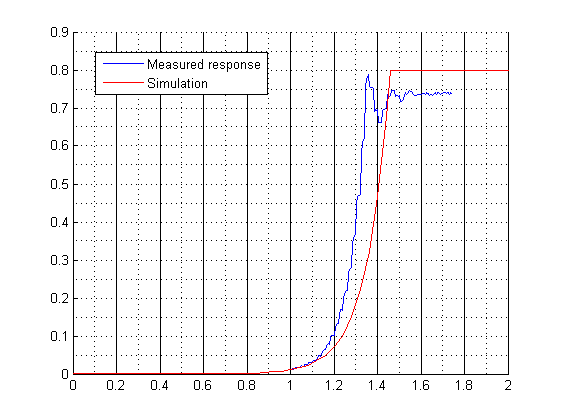
\includegraphics[scale=0.9]{figures/comparisonRealModel}
	\caption{Comparison between the real behavior and the simulation of the linearized model}
	\label{comparisonRealModel}
\end{figure} 

\subsubsection{Conclusions}